\documentclass[10pt]{book}

%These tell TeX which packages to use.
\usepackage{array,epsfig}
\usepackage{amsmath}
\usepackage{amsfonts}
\usepackage{amssymb}
\usepackage{amsxtra}
\usepackage{amsthm}
\usepackage{mathrsfs}
\usepackage{color}
\usepackage{enumitem}
%\usepackage{mdframed}
\usepackage[most]{tcolorbox}
\usepackage{pgfplots}
\pgfplotsset{compat=1.6}

\pgfplotsset{soldot/.style={color=black,only marks,mark=*}} \pgfplotsset{holdot/.style={color=black,fill=white,only marks,mark=*}}

%Here I define some theorem styles and shortcut commands for symbols I use often
\theoremstyle{definition}
\newtheorem{defn}{Definition}
\newtheorem{thm}{Theorem}
\newtheorem{cor}{Corollary}
\newtheorem*{rmk}{Remark}
\newtheorem{lem}{Lemma}
\newtheorem*{joke}{Joke}
\newtheorem{ex}{Example}
\newtheorem*{soln}{Solution}
\newtheorem{prop}{Proposition}

\newcommand{\lra}{\longrightarrow}
\newcommand{\ra}{\rightarrow}
\newcommand{\surj}{\twoheadrightarrow}
\newcommand{\graph}{\mathrm{graph}}
\newcommand{\bb}[1]{\mathbb{#1}}
\newcommand{\Z}{\bb{Z}}
\newcommand{\Q}{\bb{Q}}
\newcommand{\R}{\bb{R}}
\newcommand{\C}{\bb{C}}
\newcommand{\N}{\bb{N}}
\newcommand{\M}{\mathbf{M}}
\newcommand{\m}{\mathbf{m}}
\newcommand{\MM}{\mathscr{M}}
\newcommand{\HH}{\mathscr{H}}
\newcommand{\Om}{\Omega}
\newcommand{\Ho}{\in\HH(\Om)}
\newcommand{\bd}{\partial}
\newcommand{\del}{\partial}
\newcommand{\bardel}{\overline\partial}
\newcommand{\textdf}[1]{\textbf{\textsf{#1}}\index{#1}}
\newcommand{\img}{\mathrm{img}}
\newcommand{\ip}[2]{\left\langle{#1},{#2}\right\rangle}
\newcommand{\inter}[1]{\mathrm{int}{#1}}
\newcommand{\exter}[1]{\mathrm{ext}{#1}}
\newcommand{\cl}[1]{\mathrm{cl}{#1}}
\newcommand{\ds}{\displaystyle}
\newcommand{\vol}{\mathrm{vol}}
\newcommand{\cnt}{\mathrm{ct}}
\newcommand{\osc}{\mathrm{osc}}
\newcommand{\LL}{\mathbf{L}}
\newcommand{\UU}{\mathbf{U}}
\newcommand{\support}{\mathrm{support}}
\newcommand{\AND}{\;\wedge\;}
\newcommand{\OR}{\;\vee\;}
\newcommand{\Oset}{\varnothing}
\newcommand{\st}{\ni}
\newcommand{\wh}{\widehat}
%Pagination stuff.
\setlength{\topmargin}{-0.75in}
\setlength{\oddsidemargin}{0in}
\setlength{\evensidemargin}{0in}
\setlength{\textheight}{9.in}
\setlength{\textwidth}{6.5in}
\pagestyle{empty}
\begin{document}
\begin{flushleft}
Name:\underline{\hspace{13cm}}Date:\underline{\hspace{2cm}}
\end{flushleft}
\begin{center}
{\Large Math 1041-012 \hspace{0.5cm} Section 2.2: The Limit of a Function}
\end{center}
%\vspace{0.2 cm}

\begin{tcolorbox}
\subsection*{What is a limit?}
\begin{enumerate}
    \item A way to describe the behavior of a function $y=f(x)$ near a point $x=a$. We are not looking at what $f(a)$ is exactly!
    \item $f(x)$ needs to be defined \textit{near} the location of $x=a$
    \item We write
    \[
    \lim_{x\rightarrow a}f(x)= L
    \]
    reads as ``the limit of $f(x)$ as $x$ \underline{approaches} the value $a$ equals $L$''
    \item Imagine walking close to the location $a$ but not getting exactly on it, how is the function behaving as you get close to $a$?
\end{enumerate}
\end{tcolorbox}
\subsection*{Intro. Example}
Examine the graph of $y=x^2-x+2$ and its corresponding table of values, how does the function behave (same as asking how does $y$ behave) as $x$ approaches the value $2$? Write it in words and then in limit notation!!
\begin{figure}[h!]
\centering
    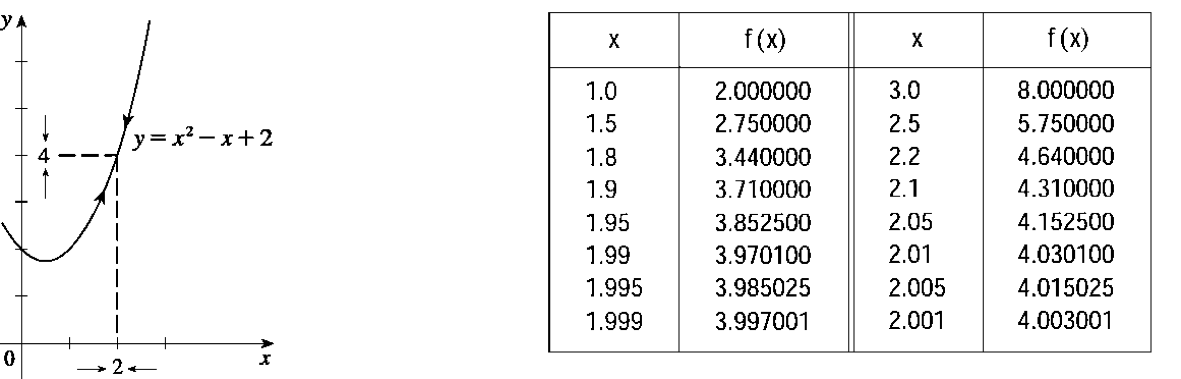
\includegraphics[scale=0.65]{fig1.png}
\end{figure}
\\ \\
\subsection*{Example 1: Take a guess?}
Guess the value of $\displaystyle \lim_{x\rightarrow 0}\frac{\sin x}{x}$.
\begin{figure}[h!]
    \centering
    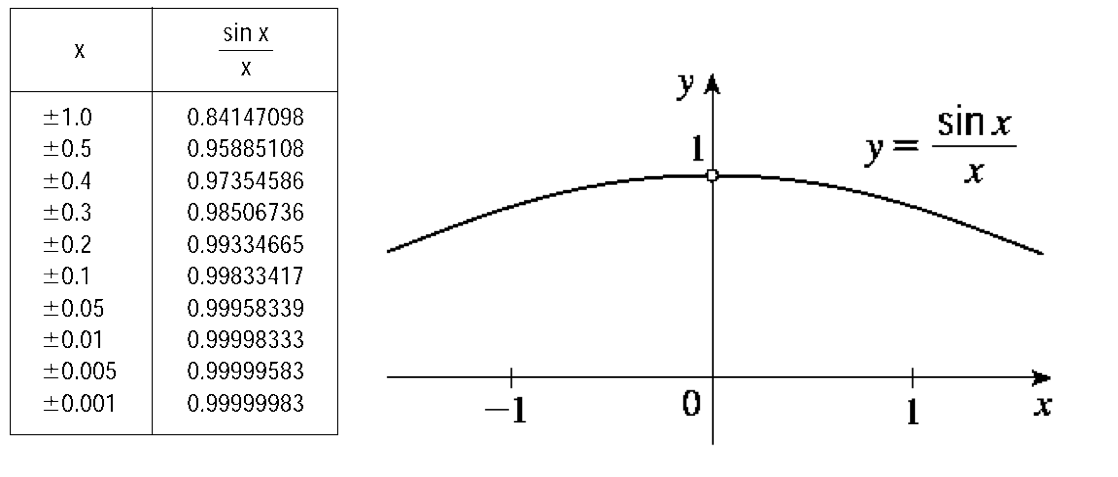
\includegraphics[scale=0.5]{fig2.png}
\end{figure}
\clearpage
\subsection*{Example 2: Does Guessing Always Work???}
Investigate $\displaystyle \lim_{x\rightarrow 0}\sin\frac{\pi}{x}$.\\
\begin{table}[h!]
    \centering
    \begin{tabular}{l|c}
        $x$&$\sin\frac{\pi}{x}$  \\
        \hline
        1 & \\[8pt]
        1/2 & \\[8pt]
        1/3 & \\[8pt]
        1/4 & \\[8pt]
        1/10 & \\[8pt]
        1/100 & \\[8pt]
        1/1000 & 
    \end{tabular}
    \quad
    \hspace{1in}
    \begin{tabular}{l|c}
        $x$&$\sin\frac{\pi}{x}$  \\
        \hline
        2 & \\[8pt]
        2/3 & \\[8pt]
        2/5 & \\[8pt]
        2/7 & \\[8pt]
        2/9 & \\[8pt]
        2/11 & \\[8pt]
        2/13 & 
    \end{tabular}
\end{table}
\\ \\ \\
\begin{tcolorbox}
\subsection*{One-Sided Limits}
\begin{itemize}
    \item $\displaystyle\lim_{x\rightarrow a^+}f(x)=L$, reads as ``the limit of $f(x)$ as $x$ approaches $a$ from the right''
    \item $\displaystyle\lim_{x\rightarrow a^-}f(x)=L$, reads as ``the limit of $f(x)$ as $x$ approaches $a$ from the left''
\end{itemize}
\subsection*{Definition}
\[
\lim_{x\rightarrow a}f(x)=L \textrm{ if and only if } \lim_{x\rightarrow a^+}f(x)=L\textrm{  \textbf{AND} }\lim_{x\rightarrow a^-}f(x)=L
\]
\end{tcolorbox}
\subsection*{Example 3: Finding Limits from a Graph}
The graph of a function $g$ is shown in the figure. Use it to state the values (if they exist) of the following:
\begin{table}[h!]
    \centering
    \begin{tabular}{ccc}
         $\displaystyle\lim_{x\rightarrow 2^-}g(x)\qquad\qquad\qquad$& $\displaystyle\lim_{x\rightarrow 2^+}g(x)\qquad\qquad\qquad$ & $\displaystyle\lim_{x\rightarrow 2}g(x)\qquad\qquad\qquad$  \\[12pt]
         $\displaystyle\lim_{x\rightarrow 5^-}g(x)\qquad\qquad\qquad$ & $\displaystyle\lim_{x\rightarrow 5^+}g(x)\qquad\qquad\qquad$ & $\displaystyle\lim_{x\rightarrow 5}g(x)\qquad\qquad\qquad$
    \end{tabular}
\end{table}
\begin{figure}[h!]
    \centering
    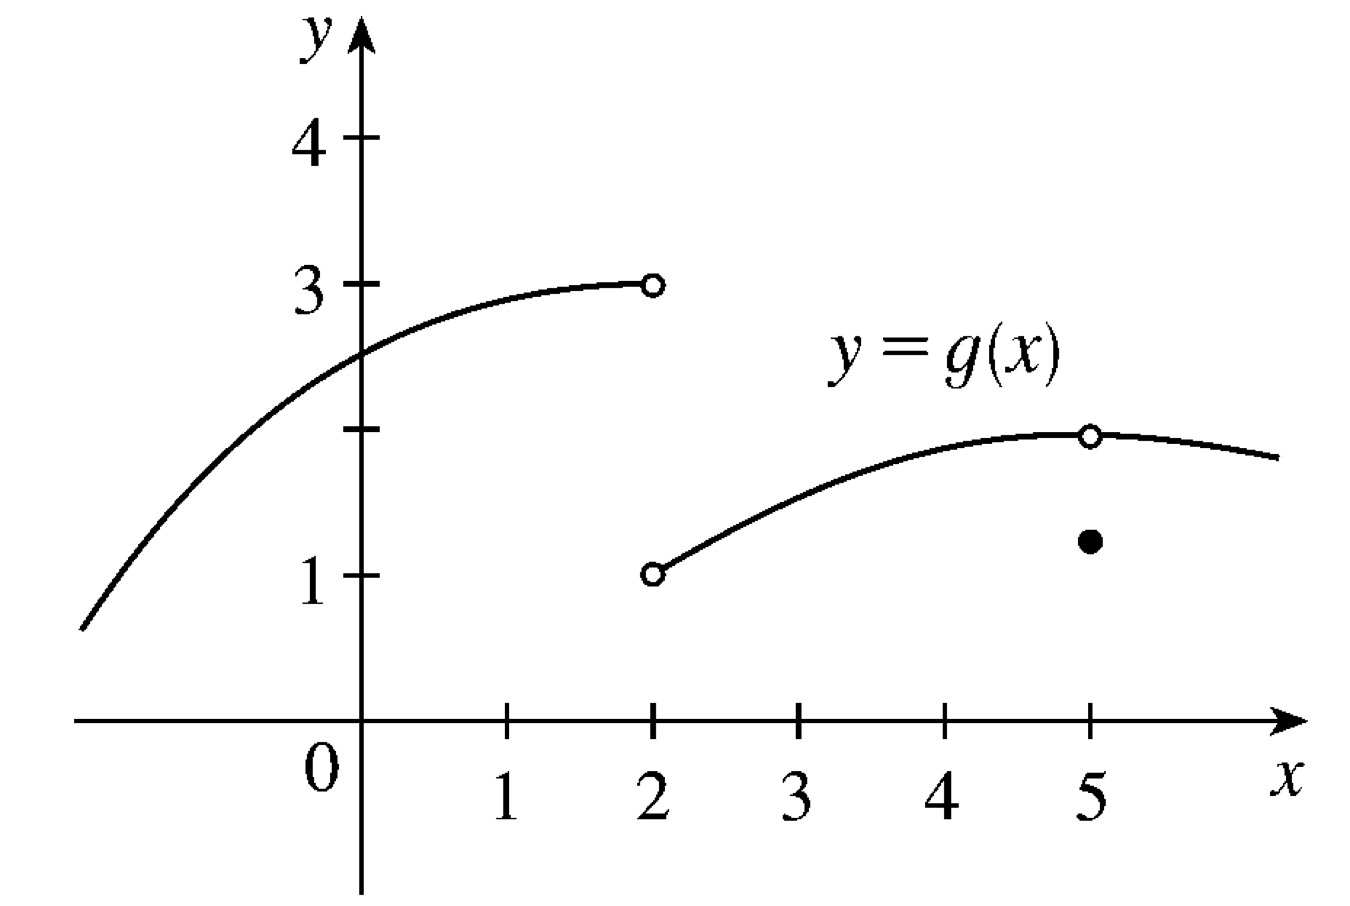
\includegraphics[scale=0.3]{fig3.png}
\end{figure}
\clearpage
\subsection*{Example 4: Infinite Limits} Find $\displaystyle\lim_{x\rightarrow 0}\frac{1}{x^2}$ if it exists!
\begin{figure}[h!]
    \centering
    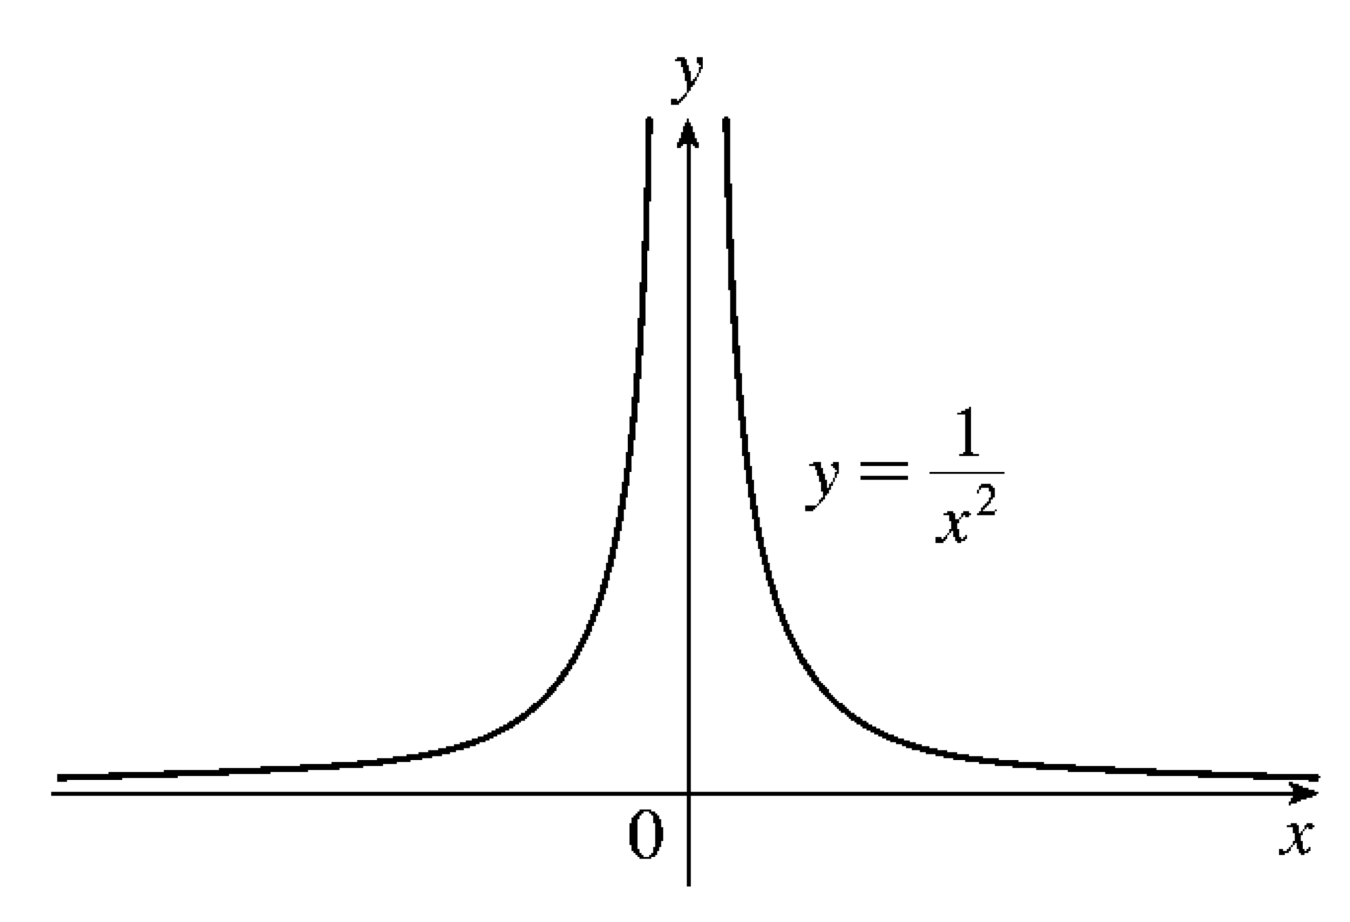
\includegraphics[scale=0.3]{fig4.png}
\end{figure}
\\ \\
\begin{tcolorbox}{What are Infinite Limits?}
\begin{itemize}
    \item These are limits where $\displaystyle\lim_{x\rightarrow a}f(x)= \infty$ or $\displaystyle\lim_{x\rightarrow a}f(x)= -\infty$
    \item THIS DOES NOT MEAN $\infty$ IS A NUMBER
    \item THIS DOES NOT MEAN THE LIMIT EXISTS, this only describes the \underline{behavior} of the function
    \item A limit exists \underline{if} both one sided limits exist and equal the same number!
\end{itemize}
\end{tcolorbox}
\subsection*{Vertical Asymptotes}
\textbf{Definition}: The line $x=a$ is a \textit{vertical asymptote} of the curve $y=f(x)$ if $\displaystyle\lim_{x\rightarrow a}f(x)=\infty$ or $\displaystyle\lim_{x\rightarrow a}f(x)=-\infty$ or one of the following occur:

\begin{figure}[h!]
    \centering
    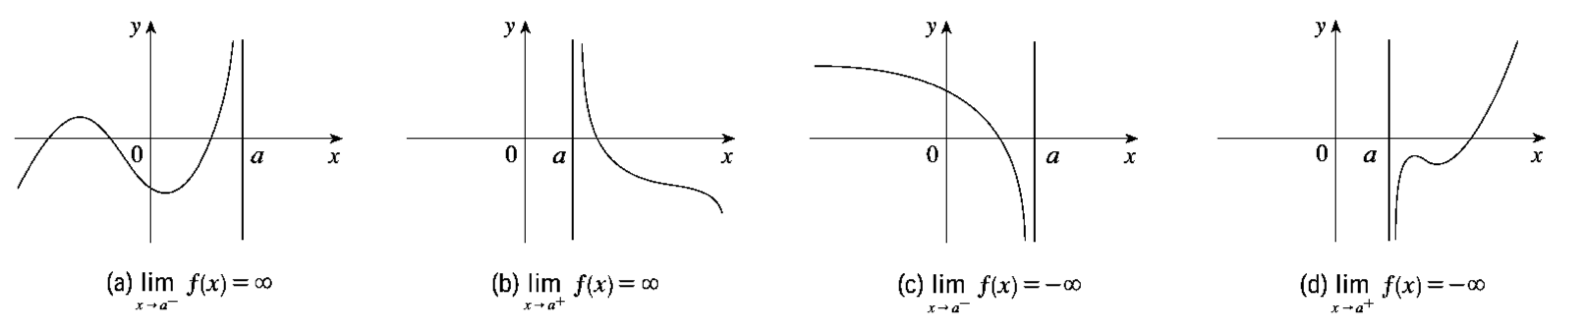
\includegraphics[scale=0.65]{fig5.png}
\end{figure}

\subsection*{Example 5: Sketching} Sketch: A function $f(x)$ where $\displaystyle\lim_{x\rightarrow 0^+}f(x)=\infty$ and $\displaystyle\lim_{x\rightarrow 0^-}f(x)=-\infty$. Can you think of an actual function that does this?
\clearpage
\subsection*{Example 6: Some practice}
\begin{itemize}
    \item[(a)] Find $\displaystyle\lim_{x\rightarrow 3^+}\frac{2x}{x-3}$ and  $\displaystyle\lim_{x\rightarrow 3^-}\frac{2x}{x-3}$. Make a rough sketch of this function!!\vspace{3in}
    \item[(b)] Find the vertical asymptotes of $f(x)=\tan x$. Make a sketch!\vspace{3in}
    \item[(c)] Sketch $y=\ln x$. Does it have any asymptote(s)? Write a limit that goes with the asymptote(s)!
\end{itemize}
\end{document}